\subsection{Kiến trúc hệ thống}

SmartDroneDelivery áp dụng Layered Architecture, trong đó các thành phần được tổ chức thành các lớp riêng biệt nhưng cùng triển khai trong một hệ thống Flask.

\begin{itemize}

\item \textbf{Presentation Layer:} Sử dụng ReactJS cho Web Manager và Flutter cho Mobile App. Các ứng dụng giao tiếp với Backend thông qua RESTful API.



\item \textbf{API \& Business Logic Layer:} Sử dụng Python/Flask, tổ chức API bằng Blueprint theo các module xác thực, người dùng, khách hàng, đơn hàng, kiện hàng, drone, trạm, thông báo, analytics và AI. Lớp này xử lý nghiệp vụ hiện đã có trong Backend; các chức năng tracking realtime và Dashboard theo từng vai trò chưa hoàn thiện trên frontend.

\item \textbf{Data Layer:} Sử dụng PostgreSQL trên Supabase, truy cập qua Flask-SQLAlchemy. Địa chỉ và trạm hiện lưu vĩ độ/kinh độ dạng số; PostGIS, MinIO và lưu file bằng chứng chưa được triển khai trong phiên bản hiện tại.

\item \textbf{AI Integration:} Backend Flask đã tích hợp Gemini cho ETA, Chatbot và tóm tắt giao hàng. Groq chưa được sử dụng trong code hiện tại.

\item \textbf{External Services:} Backend có Flask-SocketIO cho các sự kiện realtime ở mức nền tảng. Map API, Firebase Cloud Messaging (FCM) và các adapter lưu trữ bên ngoài chưa được triển khai.

\end{itemize}

\begin{figure}[H]

\centering

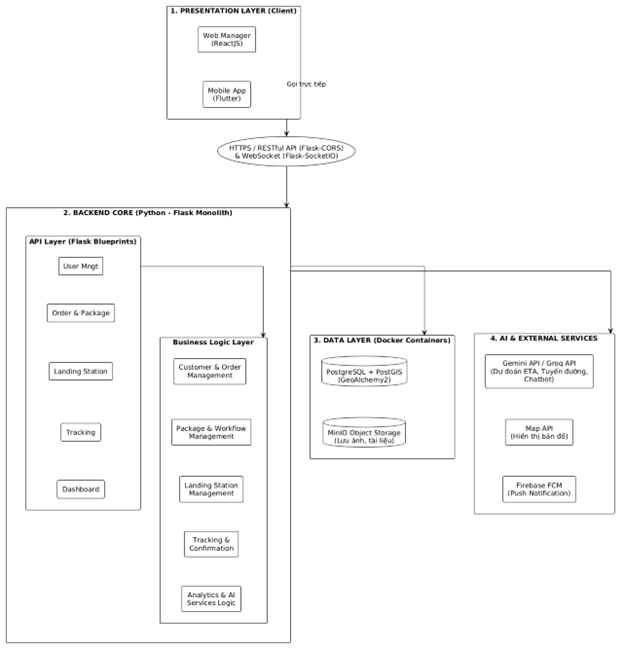
\includegraphics[width=5.88239in,height=7.12401in,keepaspectratio,width=\linewidth]{images/Sơ đồ kiến trúc hệ thống.png}

\caption{Sơ đồ kiến trúc hệ thống}
\label{fig:kien-truc-he-thong}

\end{figure} 